\documentclass{article}
\usepackage{graphicx} % Required for inserting images

\title{Labwork 3 Advanced Programming for HPC}
\author{Ta Quang Hieu - M22ICT002}
\date{October 2023}

\begin{document}

\maketitle

\section{The problem}
Labwork 3: Hello, CUDA! 
\newline
Make image RGB-to-gray converter using Numba CUDA
\begin{enumerate}
    \item Load an image from file (matplotlib’s imread)
    \item Flatten image into 1D array of RGB (reshape(pixelCount, 3))
    \item Implement grayscale using CPU (for range)
    \item Implement grayscale using GPU
    \item Save/show the image after each grayscale to validate the result visually
\end{enumerate}
Use time.time() to measure speedup

Figure ~\ref{fig:python} the image that I used in this labwork:

\begin{figure}
  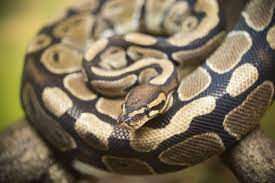
\includegraphics[width=\linewidth]{python.jpg}
  \caption{A python in rgb.}
  \label{fig:python}
\end{figure}

\section{Using CPU}
This is the script that I had used to convert an image from RGB to grayscale. Basically, I create a new grayscale image by take the average from the red, green and blue channel. The running time using GPU is \textbf{0.0004673004150390625} seconds
\begin{verbatim}
img = plt.imread('python.jpg')
red = img[:, :, 0]
green = img[:, :, 1]
blue = img[:, :, 2]

start_time = time.time()

# convert image to grayscale
gray_img = (red + green + blue)/3

cpu_time = time.time() - start_time
\end{verbatim}

Figure ~\ref{fig:cpu_python} is the result produced by CPU:

\begin{figure}
  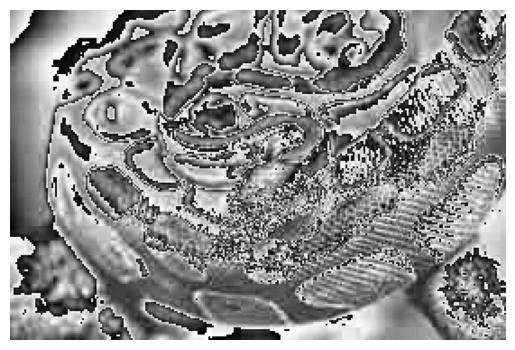
\includegraphics[width=\linewidth]{cpu_python.png}
  \caption{A grayscale python - using cpu.}
  \label{fig:cpu_python}
\end{figure}


\section{Using GPU}
This is the kernel that I had used to convert an image to grayscale using GPU:
\begin{verbatim}
# Define a Numba CUDA kernel for grayscale conversion
@cuda.jit
def grayscale(src, dst):
    # where are we in the input?
    tidx = cuda.threadIdx.x + cuda.blockIdx.x * cuda.blockDim.x
    g = np.uint8((src[tidx, 0] + src[tidx, 1] + src[tidx, 2]) / 3)
    dst[tidx, 0] = dst[tidx, 1] = dst[tidx, 2] = g
\end{verbatim}
The part \textbf{@cuda.jit} shows that this is a kernel that will be executed by the GPU. And basically what it does it just like the previous part in CPU, where we take the average of the channels. Below is the script to convert to grayscale using GPU with the running time of \textbf{0.1298370361328125} seconds:

\begin{verbatim}
# Define a Numba CUDA kernel for grayscale conversion
@cuda.jit
def grayscale(src, dst):
    # where are we in the input?
    tidx = cuda.threadIdx.x + cuda.blockIdx.x * cuda.blockDim.x
    g = np.uint8((src[tidx, 0] + src[tidx, 1] + src[tidx, 2]) / 3)
    dst[tidx, 0] = dst[tidx, 1] = dst[tidx, 2] = g
\end{verbatim}

Figure ~\ref{fig:gpu_python} is the result produced by GPU:

\begin{figure}
  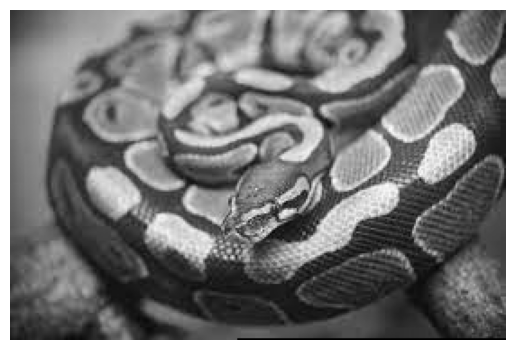
\includegraphics[width=\linewidth]{gpu_python.png}
  \caption{A grayscale python - using gpu.}
  \label{fig:gpu_python}
\end{figure}

\subsection{Block size vs time}
This is the result that I take block size from 2\^1 to 2\^9:
\begin{verbatim}
[0.08243799209594727,
 0.0013549327850341797,
 0.0007569789886474609,
 0.0008955001831054688,
 0.0006525516510009766,
 0.0006351470947265625,
 0.0006105899810791016,
 0.0006227493286132812,
 0.0008649826049804688]
\end{verbatim}
Which will turn to a plot like in Figure ~\ref{fig:plot}:
\begin{figure}
  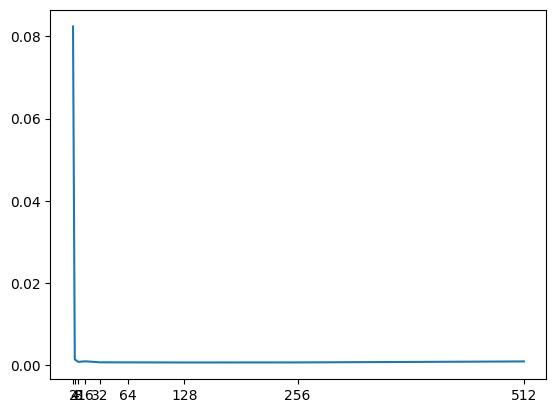
\includegraphics[width=\linewidth]{plot.png}
  \caption{A grayscale python - using gpu.}
  \label{fig:plot}
\end{figure}

\end{document}
